%%
%% licence       kaneton licence
%%
%% project       kaneton
%%
%% file          /home/mycure/kaneton/view/papers/assignments/k1.tex
%%
%% created       matthieu bucchianeri   [tue feb  7 11:49:38 2006]
%% updated       julien quintard   [sat feb 25 18:12:50 2006]
%%

%
% k1
%

\section{k1}

%
% overview
%

\subsection{Overview}

XXX

%
% description
%

\subsection{Description}

The \textbf{k1} project consists in the development of the bootloader.

This  bootloader relocates  the  stuffs needed  by  the future  kernel
execution, allocate  a bunch of memory for  kernel initialization, and
provides to the kernel a complete initialization structure.

The relocation is not really necessary but we wanted the students
to understand low-level programming and more especially programming
in a very strict environment with no fine-grain allocator provided.

So in this project, the student has to write the entire code of the
bootloader. The only requirement is to be compliant with the structure
passed to the kernel.

Students also  have to write a  tiny console driver. Try  to make this
driver code generic so you can reuse it in the next steps.

The initialization structure called \textbf{t\_init} is defined in the
file \textit{core/include/kaneton/init.h}.

\begin{verbatim}
typedef struct
{
  t_paddr                       mem;
  t_psize                       memsz;

  t_paddr                       kcode;
  t_psize                       kcodesz;

  t_paddr                       init;
  t_psize                       initsz;

  t_modules*                    modules;
  t_psize                       modulessz;

  t_uint32                      nsegments;
  o_segment*                    segments;
  t_psize                       segmentssz;

  t_uint32                      nregions;
  o_region*                     regions;
  t_psize                       regionssz;

  t_paddr                       kstack;
  t_psize                       kstacksz;

  t_paddr                       alloc;
  t_psize                       allocsz;

  machdep_data(init);
}                               t_init;
\end{verbatim}

The \textbf{mem} and \textbf{memsz} fields indicate the available physical
memory of the system.

The \textbf{kcode} and \textbf{kcodesz} fields indicate the location and
size of the kernel binary in main memory (after relocation !).

The \textbf{init} and \textbf{initsz} fields indicate the location and
size of this init structure in main memory.

The \textbf{modules} and \textbf{modulessz} fields indicate the
location of the area used to store the modules.

The modules area is composed of:

\begin{enumerate}
  \item
    The number of modules: a \textbf{t\_modules} structure.
  \item
    An array  of modules descriptors  (\textbf{t\_module}), containing
    its size and a pointer to its name
  \item
    The modules
\end{enumerate}

Each module is composed of:

\begin{enumerate}
  \item
    The module's data: binary, text etc.. depending on the module nature.
  \item
    The module name terminated by a zero character.
\end{enumerate}

Be  careful:  the   array  of  modules  is  a   variable  length  item
array. Module data and name are variable length blocks. You must refer
to the module descriptors to browse throught the modules.

The  \textbf{nsegments},   \textbf{segments}  and  \textbf{segmentssz}
fields indicate  the area location containing the  segment array. This
array describes the core's  pre-reserved segments. For the bootloader,
the  only required  fields of  the \textbf{o\_segment}  structures are
\textbf{address}, \textbf{size} and  \textbf{perms}. Other fields will
be filled at kernel initialize time.

The \textbf{nregions},  \textbf{regions} and \textbf{regionssz} fields
indicate  the area location  containing the  region array.  This array
describes the  segments to be  mapped after the initialisation  of the
core   region   manager.   You   must   fill   the   \textbf{address},
\textbf{offset} and \textbf{size} fields of each structure.

Indeed, many segments will be needless so this array only specify the
fundamental segments to map.

The \textbf{kstack} and \textbf{kstacksz} fields indicate the kernel
stack area location.

The \textbf{alloc}  and \textbf{allocsz} fields  indicate the location
and size  of the fine-grain allocator  survey area. This  area will be
used by  the \textbf{malloc()}  suite functions to  provide fine-grain
allocator  while no  segment  neither region  manager are  initialised
yet. You may allocate about 16 pages.

The  init  structure   also  contains  machine-dependent  fields,  the
\textbf{gdt} and the \textbf{page-directory}  if needed.  See the file
\textit{core/include/arch/[arch]/kaneton/init.h}  for  this  structure
(called \textbf{d\_init}).

The code provided must be located in the directory
\textit{core/bootloader/arch/[architecture]/}.

The students should use the system defines. Be aware that this project
must lead students to understand the project source organisation.

The student will have to build the init structure using the minimum
of memory, the goal of the game being to pack this structure.

Try to  think about a  very simple memory allocator  delivering single
pages or contiguous areas.

Assume that  the kernel is the  first given module.  Before jumping to
its  code,  you   must  switch  to  a  new   stack  reserved  for  the
kernel.  Remember that  switching system  stack in  a  single function
makes  impossible to  access previously  declared local  variables and
function arguments. So you will need global variables.

The kernel  should never return  after its call.  But as there  can be
loading  errors  or  code  errors,  you  must  suppose  that  it  will
return. In this case, you have to restore the old (bootloader's) stack
and display an error message.

Displaying  module  names, sizes  and  relocation  information is  the
minimum  requirement.   Having  an  enhanced display  of  pre-reserved
segments and regions will be very appreciated, but is not required.

%
% ia32
%

\subsection{IA-32 implementation}

The physical memory layout for the Intel architecture is the following:

\centerline{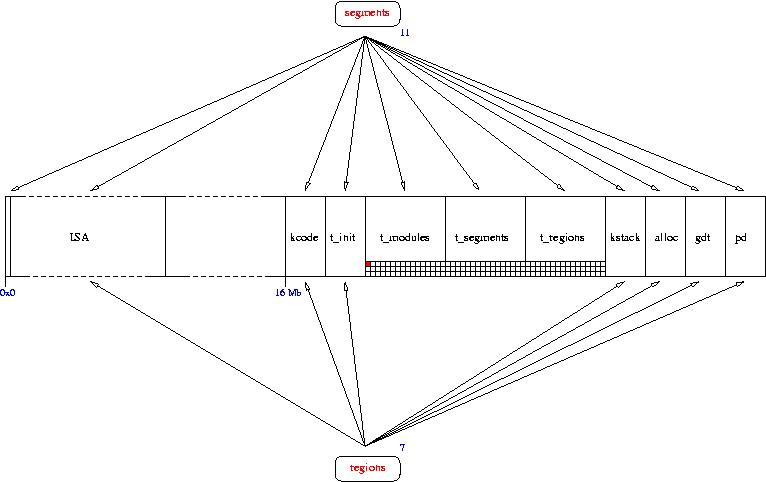
\includegraphics[scale=0.5]{figures/k1-memory-layout.jpg}}

All the segments must be mapped at the kernel boot time.

Notice that the  very first page \textbf{must not}  be mapped. Mapping
this page will cause null pointers to be valid !

Be careful to correctly initialise the machine-dependent fields
including \textbf{gdt} and \textbf{pd} which will be used by the microkernel
to retrieve the structures in main memory.

For this project,  you have to choose between using  paging or not. Be
careful:  once  this choice  done,  you  must  keep it  for  following
projects.

Here are the two possibilities:

\begin{itemize}
\item ia32-virtual, where you use paging
\item ia32-segment, without paging
\end{itemize}

---

Needless to  say, the  student will have  to install and  activate the
protected mode and the  virtual memory (students choosing ia32 without
paging will have to find an alternative to virtual memory).

Even if  the multi-bootloader  (GRUB for example)  activated protected
mode, you must ensure that it is correctly installed.

